\documentclass[british, 12pt]{article}

\usepackage[utf8]{inputenc}
\usepackage{makeidx}
\usepackage{multicol}
\usepackage{graphicx}
\graphicspath{{./images/}{./images/screenshots/}{./process-maps/}{../../static/images}}
\usepackage{caption}
\usepackage{wrapfig}
\usepackage[pdftex, 
	    bookmarks=true, 
	    colorlinks=true,
	    linkcolor=black,
	    urlcolor=blue,
	    citecolor=black,
	    anchorcolor=blue]{hyperref}
\usepackage[]{geometry}
\geometry{a4paper}
\usepackage[x11names, rgb]{xcolor}
\usepackage{tikz}
\usetikzlibrary{snakes,arrows,shapes}
\usepackage{amsmath}
\usepackage[most]{tcolorbox}
\usepackage[tikz]{bclogo}
\usepackage{varioref}
\usepackage{listings}

% \setcounter{secnumdepth}{3}
% \setcounter{tocdepth}{3}

\newcommand{\orpheusversion}{1.0}

%ideas for tip boxes: https://tex.stackexchange.com/questions/66820/how-to-create-highlight-boxes-in-latex

\newtcolorbox{tip}[1][]{
%   parbox=false,
  title=\bclampe\ \raisebox{0.5\height}{{\bfseries #1}},
  colback=blue!5!white, 
  colbacktitle=blue!20!white, 
  coltitle=black,
}

\newtcolorbox{warn}[1][]{enhanced,
  before skip=2mm,after skip=3mm,
  boxrule=0.4pt,left=5mm,right=2mm,top=1mm,bottom=1mm,
  colback=yellow!50,
  colframe=yellow!20!black,
  sharp corners,rounded corners=southeast,arc is angular,arc=3mm,
  underlay={%
    \path[fill=tcbcol@back!80!black] ([yshift=3mm]interior.south east)--++(-0.4,-0.1)--++(0.1,-0.2);
    \path[draw=tcbcol@frame,shorten <=-0.05mm,shorten >=-0.05mm] ([yshift=3mm]interior.south east)--++(-0.4,-0.1)--++(0.1,-0.2);
    \path[fill=yellow!50!black,draw=none] (interior.south west) rectangle node[white]{\Huge\bfseries !} ([xshift=4mm]interior.north west);
    },
  drop fuzzy shadow,#1}
  
% \newenvironment{tip}{\begin{tcolorbox}[colback=black!5!white, colbacktitle=black!20!white, coltitle=black, title=Tip]}{\end{tcolorbox}}

% \pdfinfo{%
%   /Title    ()
%   /Author   ()
%   /Creator  ()
%   /Producer ()
%   /Subject  ()
%   /Keywords ()
% }

\tikzstyle{help lines}=[red!50,very thin]

%%%%%%%%%%%%%%%%%%%%%%%%%%%%%%%%%%%%%%%%%%%%%%%%%%%%%%%%%%%%%%%%%%%%%%
% LaTeX Overlay Generator - Annotated Figures v0.0.1
% Created with http://ff.cx/latex-overlay-generator/
% If this generator saves you time, consider donating 5,- EUR! :-)
%%%%%%%%%%%%%%%%%%%%%%%%%%%%%%%%%%%%%%%%%%%%%%%%%%%%%%%%%%%%%%%%%%%%%%
%\annotatedFigureBoxCustom{bottom-left}{top-right}{label}{label-position}{box-color}{label-color}{border-color}{text-color}
\newcommand*\annotatedFigureBoxCustom[8]{\draw[#5,ultra thick,rounded corners] (#1) rectangle (#2);\node at (#4) [fill=#6,thick,shape=circle,draw=#7,inner sep=2pt,font=\sffamily,text=#8] {\textbf{#3}};}
%\annotatedFigureBox{bottom-left}{top-right}{label}{label-position}
\newcommand*\annotatedFigureBox[3]{\annotatedFigureBoxCustom{#1}{#2}{#3}{#1}{black}{white}{black}{black}}
\newcommand*\annotatedFigureText[4]{\node[draw=none, anchor=south west, text=#2, inner sep=0, text width=#3\linewidth,font=\sffamily] at (#1){#4};}
\newenvironment {annotatedFigure}[1]{\centering\begin{tikzpicture}
\node[anchor=south west,inner sep=0] (image) at (0,0) { #1};\begin{scope}[x={(image.south east)},y={(image.north west)}]}{\end{scope}\end{tikzpicture}}
%%%%%%%%%%%%%%%%%%%%%%%%%%%%%%%%%%%%%%%%%%%%%%%%%%%%%%%%%%%%%%%%%%%%%%

%%% Commands for Schol Comms entities
\newcommand{\journal}[1]{\emph{#1}}
\newcommand{\imprint}[1]{\emph{#1}}
\newcommand{\publisher}[1]{\emph{#1}}

%%% Commands for Software/Applications/Files
\newcommand{\software}[1]{\emph{#1}\index{#1}}

%%% Commands for interface components
\newcommand{\dbfield}[1]{\emph{#1}\index{#1}}
\newcommand{\dbtable}[1]{\emph{#1}\index{#1}} % Database tables, such as Contacts, Licences,  Responsibilities
\newcommand{\icomponent}[1]{\textbf{#1}\index{#1}} % components of the interface: navigation bar, etc
\newcommand{\menuitem}[1]{\emph{#1}\index{#1}}
\newcommand{\viewtype}[1]{\emph{#1}\index{#1}} % list view, detail view, etc
\newcommand{\view}[1]{\emph{#1}\index{#1}} % Jounals, Publishers, Sources, etc
\newcommand{\fieldvalue}[1]{\emph{#1}\index{#1}}
\newcommand{\action}[1]{\emph{#1}\index{#1}} % action buttons, such as "add new" "edit record" etc
%%%

%%% Commands for figure captions
\newcommand{\abbv}[2]{\textbf{#1}, #2}
\newcommand{\captionindex}[1]{#1\index{#1}}

%%% Commands for standard elements
\newcommand{\figp}[1]{Fig.~#1}
\newcommand{\figt}[1]{Fig.~#1}

\makeindex

\begin{document}
\title{
\includegraphics[width=0.8\textwidth]{orpheus-logo-final}\\
  \large Manual for version \orpheusversion\\[1mm]
%\large\href{https://github.com/osc-cam/orpheus}{\texttt{https://github.com/osc-cam/orpheus}}
}
\author{André Sartori\\
  \normalsize University of Cambridge\\[-1mm]
  \normalsize Office of Scholarly Communication}
\maketitle

\tableofcontents{}

\section{Introduction}

Orpheus is a database of academic journals and their policies written in \href{https://www.djangoproject.com}{Django}. It features web frontends for users and administrators and a RESTful API, tailored for integration with DSpace and other institutional repository platforms.

\section{Installation}

\lstset{language=bash}

\subsection{Obtaining a copy of Orpheus}

You may either download and extract a zip file from \url{https://github.com/osc-cam/orpheus/archive/master.zip} or clone the git repository by issuing the following command in your UNIX terminal:

\begin{lstlisting}
  $ git clone https://github.com/osc-cam/orpheus.git
\end{lstlisting}

\subsection{Setting up a database backend}

Django supports many different database backends\footnote{see \url{https://docs.djangoproject.com/en/1.11/ref/databases} for details and notes}, which may or may not work with Orpheus out of the box. Orpheus was developed and has only been tested using a PostgreSQL backend, so this is the recommended database engine.

Once you have created an empty database in the engine of your choice\footnote{if you decide to use PostgreSQL and you are running Ubuntu or derivatives, a good guide on configuring the database is available at \url{https://www.codeproject.com/Articles/898303/Installing-and-Configuring-PostgreSQL-on-Linux-Min}. For other databases and operational systems, Google is your friend!}, you will need to edit the value of \mbox{DATABASES} in file \path{orpheus/settings_local_example.py} to match the parameters of the database you have just created.

While you are editing this file, you may also wish to change the value of \mbox{SECRET\_KEY}. If your instance of Orpheus will be reachable from outside of your local network, you should review your settings before deployment\footnote{see \url{https://docs.djangoproject.com/en/1.11/howto/deployment/checklist} for recommended settings}.

Once you have completed this, rename the file \path{orpheus/settings_local_example.py} to \path{orpheus/settings_local.py}

\subsection{Creating and activating a virtual environment (optional, but recommended)}

To create and activate new virtual environment for Orpheus, issue the following commands:

\begin{lstlisting}
  $ python3 -m venv orpheus-env
  $ source orpheus-env/bin/activate
\end{lstlisting}

\subsection{Installing the dependencies}

To install all Orpheus dependencies, navigate to the folder containing the code you downloaded or cloned from GitHub and issue the command:

 \begin{lstlisting}
  $ pip3 install -r requirements.txt
 \end{lstlisting}

\subsection{Applying migrations}

To create the database fields that Orpheus will need to store its data, apply migrations by running:

 \begin{lstlisting}
  $ python3 manage.py migrate
 \end{lstlisting}

\subsection{Creating a superuser}

You will need at least one user who can login to Orpheus, so run the following command to create it:

 \begin{lstlisting}
  $ python3 manage.py createsuperuser
 \end{lstlisting} 
 
\subsection{Testing your Installation}

You should now have a functional development instance of Orpheus! To test it, issue the command:

\begin{lstlisting}
  $ python3 manage.py runserver
 \end{lstlisting}
 
And then point your favourite browser to \url{http://127.0.0.1:8000/}. You should see Orpheus' homepage.

\subsection{Populating auxiliary tables}

Some of Orpheus' tables include fields that are populated using values stored in four small, auxiliary tables (\dbtable{Licence}, \dbtable{Outlet}, \dbtable{Responsibility} and \dbtable{Version}). Unless these four tables contain at least one value each, some of forms in the \hyperref[sec-frontend-for-editors]{frontend for editors} will not work.

To populate these four tables you may either use the \hyperref[sec-frontend-for-administrators]{frontend for administrators} or you may import the JSON files that come with the Orpheus source code by issuing the command:\footnote{for more details, see \url{https://docs.djangoproject.com/en/1.11/howto/initial-data/}}

\begin{lstlisting}
  $ python3 manage.py loaddata Licence Outlet \
    Responsibility Version
\end{lstlisting}

\subsection{Importing some data}

Unless you intend to populate the database manually, you will now probably want to bulk import some data into your Orpheus instance. The \path{connectors} folder of the Orpheus source code contains a number of Python parsers that can be used to import large datasets made available by a number of publishers and projects. Editing and running these parsers is the recommended method of bulk populating and curating the database. 

However, if you just want to load as much data as possible to your Orpheus instance for testing purposes, you may import JSON files providing a recent snapshot of most of the database hosted by the University of Cambridge. You can do so by issuing the command (it will take a while to complete):

\begin{lstlisting}
  $ python3 manage.py loaddata Source Node Deal Epmc \
    GoldPolicy GreenPolicy OaStatus
\end{lstlisting}

\section{Frontend for editors}
\label{sec-frontend-for-editors}

The Orpheus web frontend for editors is available at \url{https://orpheus-prod.lib.cam.ac.uk}. From the \view{homepage}, users can use the \icomponent{navigation bar} (\figp{\ref{fig-home}}A) to navigate to one of the \viewtype{list views} described in section \vref{sec-list-views}. The \view{homepage} also summarises the contents of database in a ``contents at a glance'' table (\figp{\ref{fig-home}}B).

% For a nice guide on figure annotation, see:
% https://tex.stackexchange.com/questions/9559/drawing-on-an-image-with-tikz/9562#9562
\begin{figure}
  \begin{tikzpicture}
    \node[anchor=south west,inner sep=0] (image) at (0,0) {\fbox{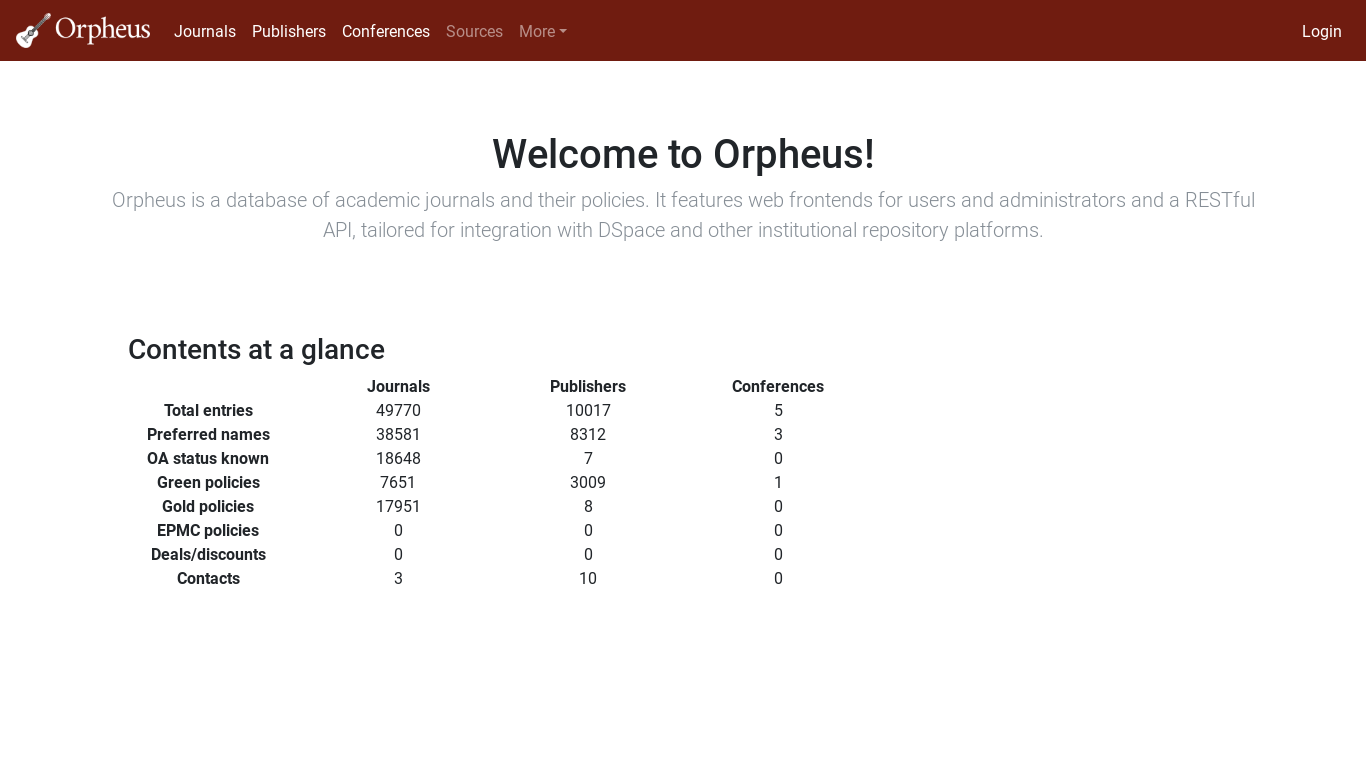
\includegraphics[width=\textwidth]{home}}};
    \begin{scope}[x={(image.south east)},y={(image.north west)}]
%       \draw[help lines,xstep=.1,ystep=.1] (0,0) grid (1,1);
%       \foreach \x in {0,1,...,9} { \node [anchor=north] at (\x/10,0) {0.\x}; }
%       \foreach \y in {0,1,...,9} { \node [anchor=east] at (0,\y/10) {0.\y}; }
      
      \annotatedFigureBox{0,0.89}{1,1}{A}
      \annotatedFigureBox{0.09,0.21}{0.61,0.6}{B}
    \end{scope}
  \end{tikzpicture}
  \caption{The main elements of the homepage. \abbv{A}{\captionindex{navigation bar}}; \abbv{B}{\captionindex{contents at a glance} table}.}
  \label{fig-home}
\end{figure}

\begin{tip}[Sandbox]
  A sandbox for testing and familiarising yourself with the database is available at \url{https://orpheus-dev.lib.cam.ac.uk}
  \vspace{1em}

  To login to the sandbox, please use the following credentials:

  username: \texttt{test\textunderscore curator}

  password: \texttt{Orpheus\textunderscore dev}
\end{tip}

\begin{warn}
 At present, Orpheus is only available on the University Libraries intranet. To access it while away from the UL, you will need to connect to the library VPN first. For instructions on how to do this, please refer to \url{https://wiki.cam.ac.uk/dspace/Connecting_to_shared_drive_while_away_from_UL}.
\end{warn}

\subsection{List views}
\label{sec-list-views}

List views allow users to browse and search for specific entries in the Orpheus database (\figp{\vref{fig-journals}}). 
For instance, \view{Journals}, \view{Publishers} and \view{Conferences} are list views displaying records of those entities.

The \icomponent{search box} on the top right corner of a \viewtype{list view} page can be used to search for records containing a particular word or string (\figp{\ref{fig-journals}}A), and the \icomponent{paginator} at the bottom of a \viewtype{list view} can be used to browse records (\figp{\ref{fig-journals}}D). List views also include an action button \action{add new}, positioned immediately to the right of the list heading. When clicked, this button takes the user to a web form where they can add a new entry.

A brief description of each available \viewtype{list view} is provided below.

\subsubsection{General list views}

\paragraph{Journals} Lists all journal records in the database, in alphabetical order.
\paragraph{Publishers} Lists all publisher records in the database, in alphabetical order.
\paragraph{Conferences} Lists all conference records in the database, in alphabetical order.
\paragraph{Sources} Lists all source records in the database, in the order they were created.\marginpar{Change to alphabetical?}

\subsubsection{Curatorial list views}

Orpheus comes with a number of lists views intended to facilitate the detection of problems and curation of the database. You will find these views under the \icomponent{navigation bar} item \menuitem{More}.

\paragraph{Problematic policies} Lists Orpheus records (journals, publishers or conferences) that contain one or more policies flagged as problematic (checkbox \dbfield{problematic} ticked). This view is sorted by descending number of children records linked to the listed records, so policies imported from RoMEO that apply to hundreds of journals will be listed at the top.

\paragraph{Children of synonyms} Lists Orpheus records in which the  \dbfield{name status} field of the parent record is not set to \fieldvalue{preferred name}. In other words,  it will typically list journals that are linked to a synonym of a publisher (e.g. OUP), rather thant the publisher's preferred name (Oxford University Press). Ideally, the parent of an Orpheus records should always be a preferred name.

\paragraph{Children of non-publisher nodes} Lists Orpheus records in which the  \dbfield{type} field of the parent record is not set to \fieldvalue{publisher}. In other words,  it will typically list journals that are catalogued as children of other journals rather than of a publisher.

\paragraph{Grandchildren} Lists Orpheus records whose parent record has a parent record. Although having grandparents could be useful to express, for example, relationships between journals, imprints and publishers (\journal{Cell} is published by \imprint{Cell Press}, an imprint of \publisher{Elsevier}), Orpheus' logic for policy inheritance does not currently support inheritance from grandparents. The negative impact on database performance of implementing another level of inheritance is probably not worth the potential benefit.

\paragraph{Synonyms of synonyms} Lists Orpheus records whose \dbfield{synonym of} field points to a journal/publisher record in which the  \dbfield{name status} field is not set to \fieldvalue{preferred name}. In other words,  it will typically list journals that are deemed synonyms of other synonyms, rather than being linked directly to the preferred name.

\paragraph{Synonyms with linked policies} Lists Orpheus records containing one or more attached policies and whose \dbfield{name status} field is not set to \fieldvalue{preferred name}.

\subsubsection{Search box behaviour}
\label{sec-search-behaviour}
Search boxes in Orpheus may be used to restrict list views to items containing a word or phrase of interest. The search engine is case insensitive, so both \journal{System analysis and applied information science} and \journal{ACS Biomaterials Science and Engineering} will be included in the results of a search for the string ``science''. Strings entered in the search box are evaluated as a whole. Thus, \journal{ACS Biomaterials Science and Engineering} will \emph{not} be included in the results of a search for ``Science Engineering".

\begin{tip}[Searching by ISSN]
  The list views \view{Journals}, \view{Publishers} and \view{Conferences} also support searches by ISSN. This can be particularly useful to quickly find journal titles consisting of short and common words, such as ``Science'' and ``Nature''.
\end{tip}



\begin{warn}
 Be careful with leading or trailing spaces when entering a string into the search box. These will be included in the search, so if you search for ``Nature '', you will \emph{not} find the journal ``Nature'' (but you will find ``Nature Astronomy'').
\end{warn}




\begin{figure}
  \begin{center}
  \begin{tikzpicture}
    \node[anchor=south west,inner sep=0] (image) at (0,0) {\fbox{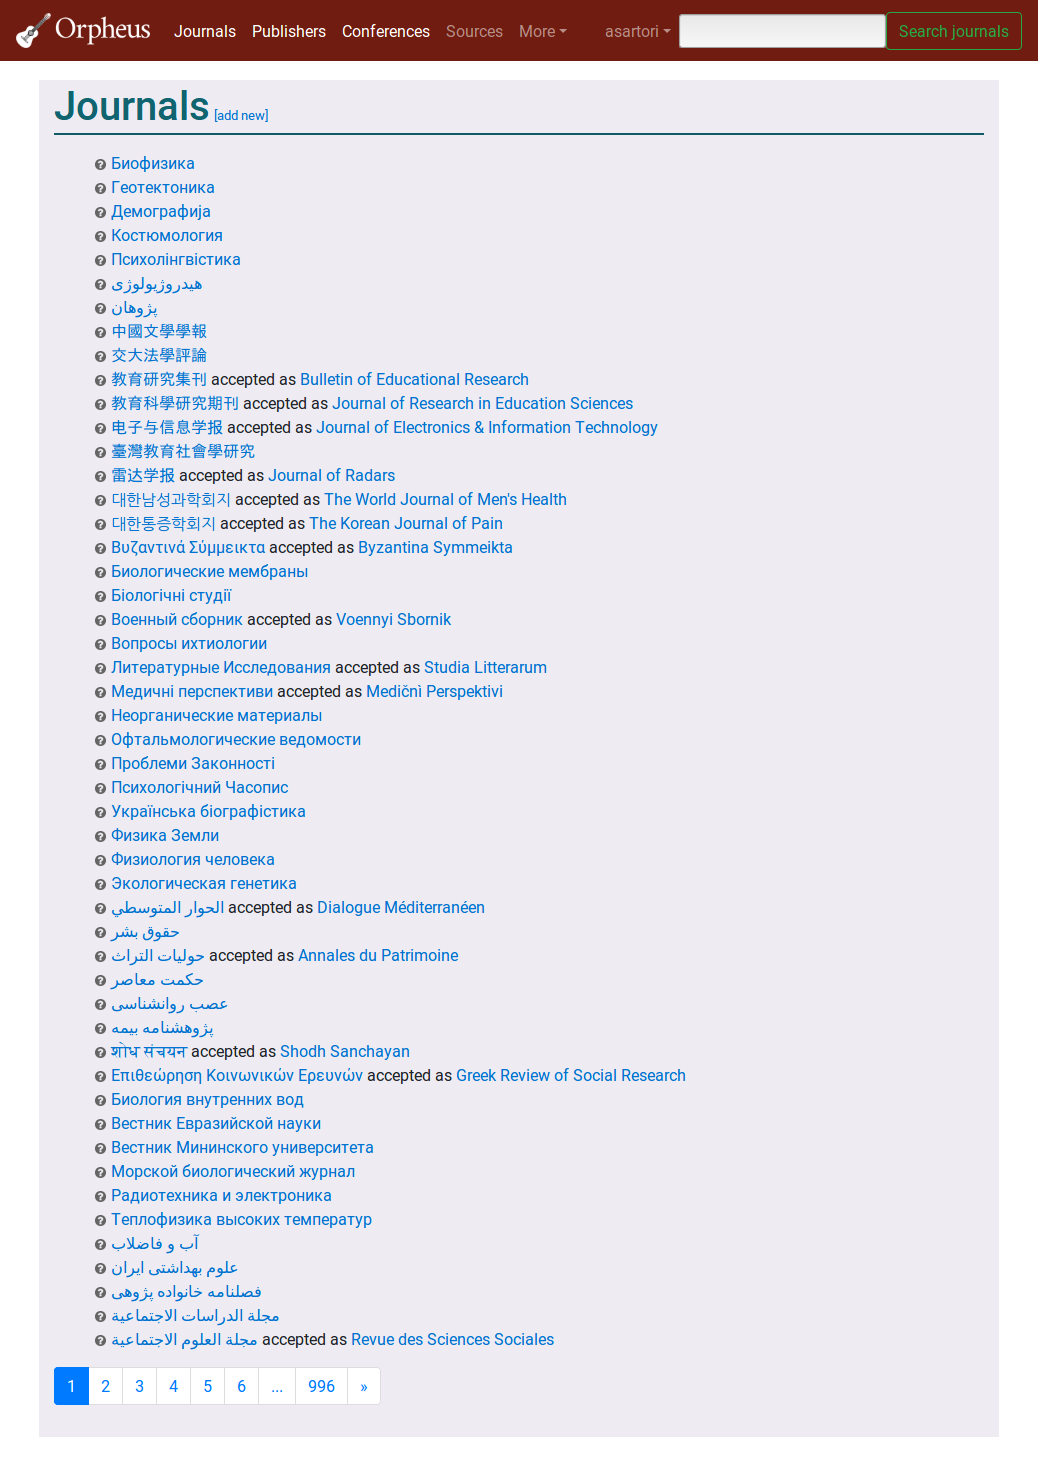
\includegraphics[width=0.9\textwidth]{journals}}};
    % screenshot journals was taken by using Firefox inbuilt screenshot feature (https://support.mozilla.org/en-US/kb/firefox-screenshots) and selecting to take a screenshot of the whole screen after making the window just big enough to allow for the navigation bar to be properly displayed. This resulted in a screenshot sized 1038x1469 pixels
    \begin{scope}[x={(image.south east)},y={(image.north west)}]
%       \draw[help lines,xstep=.1,ystep=.1] (0,0) grid (1,1);
%       \draw[help lines,dashed,xstep=.05,ystep=.05] (0,0) grid (1,1);
%       \foreach \x in {0,1,...,9} { \node [red, anchor=north] at (\x/10,0) {0.\x}; }
%       \foreach \y in {0,1,...,9} { \node [red, anchor=east] at (0,\y/10) {0.\y}; }
      \annotatedFigureBox{0.645,0.95}{1,1}{A}
      \annotatedFigureBox{0.2,0.905}{0.275,0.93}{B}
      \annotatedFigureBox{0.05,0.045}{0.375,0.08}{D}
      \annotatedFigureBox{0.09,0.0875}{0.68,0.89}{C}
    \end{scope}
  \end{tikzpicture}
  \caption{Elements of an Orpheus \viewtype{list view}. \abbv{A}{\captionindex{search box}}; \abbv{B}{``add new'' action button}; \abbv{C}{list of entries (journals in this case), showing up to 50 records}; \abbv{D}{\captionindex{paginator}}.}
  \label{fig-journals}
  \end{center}
\end{figure}

\subsection{Detail views}
\label{sec-detail-views}
If a user clicks on a record in a \viewtype{list view} they are taken to the \viewtype{detail view} of that record. A \viewtype{detail view} displays most or all data available in Orpheus for a particular record. Figure \vref{fig-journal-detail} shows the detail view of \journal{Advanced Materials}.

\begin{figure}
  \begin{center}
  \begin{tikzpicture}
    \node[anchor=south west,inner sep=0] (image) at (0,0) {\fbox{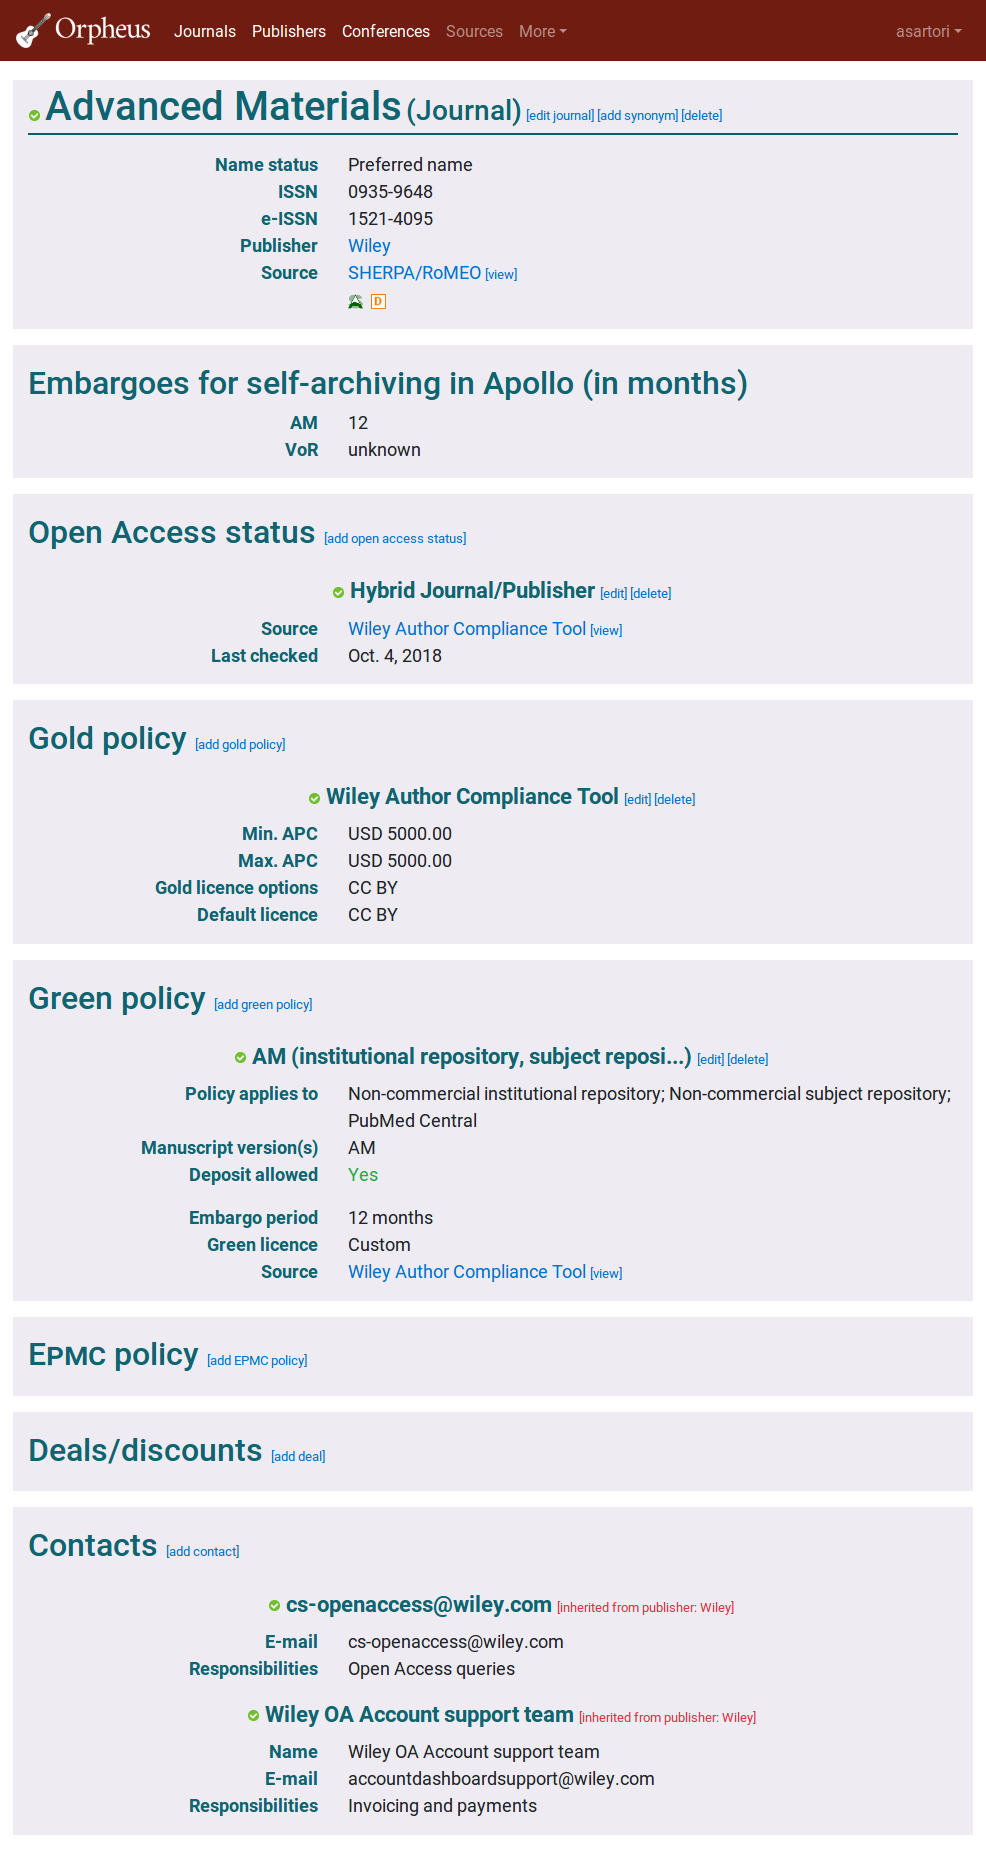
\includegraphics[width=0.7\textwidth]{journal-detail}}};
    \begin{scope}[x={(image.south east)},y={(image.north west)}]
%       \draw[help lines,xstep=.1,ystep=.1] (0,0) grid (1,1);
%       \draw[help lines,dashed,xstep=.05,ystep=.05] (0,0) grid (1,1);
%       \foreach \x in {0,1,...,9} { \node [red, anchor=north] at (\x/10,0) {0.\x}; }
%       \foreach \y in {0,1,...,9} { \node [red, anchor=east] at (0,\y/10) {0.\y}; }
%       \annotatedFigureBox{0.645,0.95}{1,1}{A}
%       \annotatedFigureBox{0.2,0.905}{0.275,0.93}{B}
%       \annotatedFigureBox{0.05,0.045}{0.375,0.08}{D}
%       \annotatedFigureBox{0.09,0.0875}{0.68,0.89}{C}
    \end{scope}
  \end{tikzpicture}
  \caption{Bird-eye view of the \viewtype{detail view} of a journal. See section \vref{sec-detail-views} for an explanation of the different elements.}
  \label{fig-journal-detail}
  \end{center}
\end{figure}


\subsection{Quality indicators}

Orpheus has a number of fields indicating the quality of data for every journal/publisher name and policy in the database:

\begin{itemize}
  \item \dbfield{Vetted}: Indicates that data was created or modified by the an editor. All data entered or edited using the Orpheus web frontend has this field ticked by default.
  \item \dbfield{Vetted date}: Automatic timestamp recording the date a record or policy was first vetted by an editor.
  \item \dbfield{Last checked}: Date a policy was last checked by an editor.
  \item \dbfield{Superseded}: Indicates that policy is no longer valid (it was probably superseded by a revised policy).
  \item \dbfield{Superseded date}: Date an editor first realised that policy is no longer valid.
  \item \dbfield{Problematic}: Indicates ambiguous/unclear policies requiring discussion/revision.
\end{itemize}

Orpheus uses the fields above to provide users with an icon that visually indicates the curation quality of data. These icons precede the main heading of each record and policy in the database (see \figp{\vref{figure-journal-inheriting-from-romeo-after-translation}} for an example of the placement) and their meaning is:

\begin{itemize}
  \item 
\includegraphics{icon-no}: Policy should not be trusted. It is either superseded or the field \dbfield{problematic} is checked.
  \item 
\includegraphics{icon-unknown}: Policy has not been vetted by an editor yet, but it can be trusted. All records and policies created during the initial bulk population of the database (see section \vref{section-bulk-import} for details) were at that point marked with this icon.
  \item 
\includegraphics{icon-yes}: Policy was vetted by editor it is not superseded nor marked as problematic. This is the highest level of quality implemented in Orpheus.
\end{itemize}

\begin{warn}
  Note that an orange question mark image (
\includegraphics{icon-unknown-orange}) is also used in Orpheus, but this is \emph{not} a quality indicator. Instead, it indicates that field \dbfield{version embargo months} is empty (unknown), just to avoid confusion with absence of embargo (\dbfield{version embargo months}=0). 
\end{warn}

\section{Frontend for administrators}
\label{sec-frontend-for-administrators}
The Orpheus web frontend for administrators, available at \url{https://orpheus-prod.lib.cam.ac.uk/admin}, provides tools for user management and editing of database tables that cannot be altered by editors (\figp{\vref{fig-admin}}). For example, new values for the tables \dbtable{Licences} and \dbtable{Outlets}, which are used to populate value lists in forms used by editors, can be added via this interface.

\begin{warn}
 Be careful when editing existing values of valuelist tables via the admin interface. Some of the values are used by API methods and altering these could break the Orpheus API. Remember that with great power comes great responsibility.
\end{warn}


\begin{figure}
  \begin{tikzpicture}
    \node[anchor=south west,inner sep=0] (image) at (0,0) {\fbox{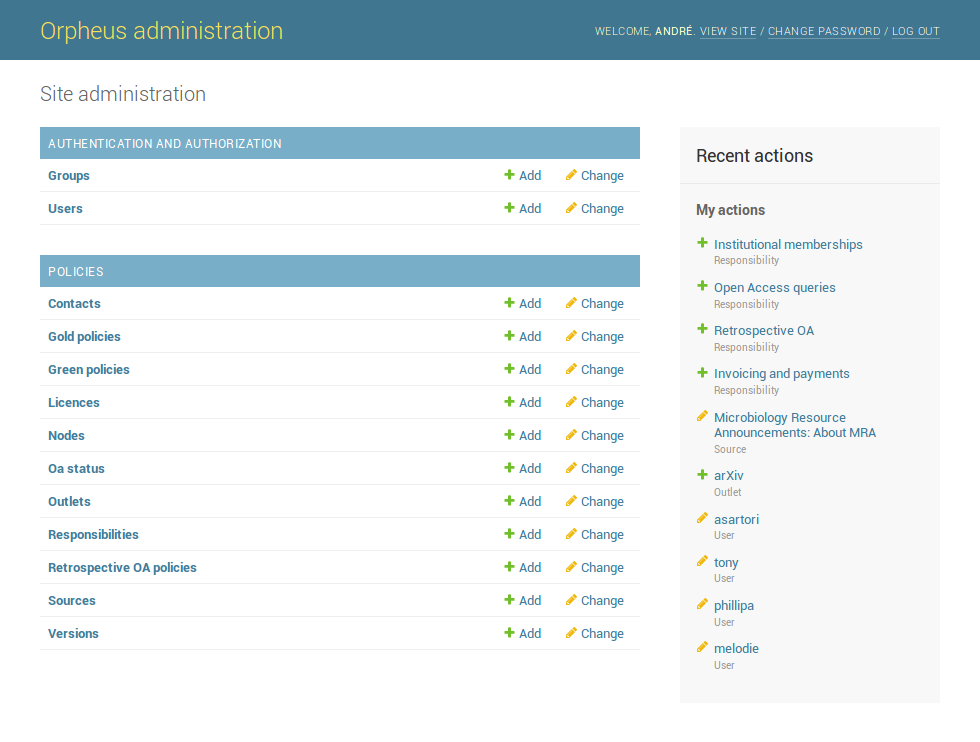
\includegraphics[width=\textwidth]{admin}}};
    % screenshot journals was taken by using Firefox inbuilt screenshot feature (https://support.mozilla.org/en-US/kb/firefox-screenshots) and selecting to take a screenshot of the whole screen after making the window just big enough to allow for the navigation bar to be properly displayed. This resulted in a screenshot sized 1038x1469 pixels
    \begin{scope}[x={(image.south east)},y={(image.north west)}]
%       \draw[help lines,xstep=.1,ystep=.1] (0,0) grid (1,1);
%       \draw[help lines,dashed,xstep=.05,ystep=.05] (0,0) grid (1,1);
%       \foreach \x in {0,1,...,9} { \node [red, anchor=north] at (\x/10,0) {0.\x}; }
%       \foreach \y in {0,1,...,9} { \node [red, anchor=east] at (0,\y/10) {0.\y}; }
%       \annotatedFigureBox{0.645,0.95}{1,1}{A}
%       \annotatedFigureBox{0.2,0.905}{0.275,0.93}{B}
%       \annotatedFigureBox{0.05,0.045}{0.375,0.08}{D}
%       \annotatedFigureBox{0.09,0.0875}{0.68,0.89}{C}
    \end{scope}
  \end{tikzpicture}
  \caption{Orpheus frontend for administrators.}
  \label{fig-admin}
\end{figure}


\section{Strategy for quickly expanding coverage of self-archiving policies}

Increasing Orpheus coverage of self-archiving policies pertaining to accepted versions deposited in institutional repositories is paramount to achieving high-quality Apollo deposits with the correct embargo period applied.

This section provides an overview of the current state of the Orpheus database regarding self-archiving (green) policies and explains how we can most efficiently use and edit Orpheus to quickly populate it with reliable embargo periods.

\subsection{Pre-populated database}
\label{section-bulk-import}

The Orpheus' database was pre-populated in August 2018 by importing a number of policies datasets from:

\begin{enumerate}
 \item \href{https://authorservices.taylorandfrancis.com/journal-list/#}{Taylor \& Francis}
 \item \href{https://doi.org/10.6084/m9.figshare.1554748.v14}{Version 14 of Andrew Gray's "Elsevier embargo periods, 2013-2018"}
 \item \href{https://www.elsevier.com/__data/promis_misc/j.custom97.pdf}{Elsevier's OA Price List}
 \item \href{https://authorservices.wiley.com/author-resources/Journal-Authors/open-access/author-compliance-tool.html}{Wiley's "Author Compliance tool"}
 \item \href{https://www.cambridge.org/core/services/aop-file-manager/file/5783738dbd8dfd4e3283c3f2}{Cambridge University Press}
 \item \href{https://academic.oup.com/journals/pages/access_purchase/rights_and_permissions/embargo_periods}{Oxford University Press}
 \item \href{https://doaj.org/}{Directory of Open Access Journals}
 \item \href{http://www.sherpa.ac.uk/romeo/index.php}{Sherpa RoMEO}
\end{enumerate}

With the exception of the Sherpa RoMEO dataset, all these data sources contain data that can be easily parsed and understood by a computer, and hence data was linked to individual journals, resulting in 18,634 journals with a known OA status (i.e.\ categorised as fully Open Access, hybrid or subscription), 7,646 with a known embargo period and 17,939 journals with a known APC value and/or gold OA licence (Table \vref{table-bulk-import}).

RoMEO data could not be reliably interpreted by a computer but RoMEO contains only 3,006 self-archiving policies, each of which linked to all applicable journals. Hence, these 3,006 policies were imported into Orpheus at the Publisher level and marked as requiring editorial revision (`problematic' field ticked). \emph{Once revision of these policies is completed, Orpheus will be able to provide reliable embargo information to Apollo for all 38,577 journals in the database, rather than the 7,646 currently covered}.

\begin{table}
\begin{center}
\caption{Overview of Orpheus database following bulk imports}
\label{table-bulk-import}
\begin{tabular}{lcc}
			&Journals 	&Publishers\\
Total entries		&49751		&10013\\
Preferred names		&38577		&8309\\
OA status known		&18634		&0\\
Green policies		&7646		&3006\\
Gold policies		&17939		&0\\
\end{tabular} 
\end{center}
\end{table} 

\subsection{General use and editing workflow}

%\begin{wrapfigure}{R}{0.5\textwidth}
\begin{figure}
  \begin{center}
     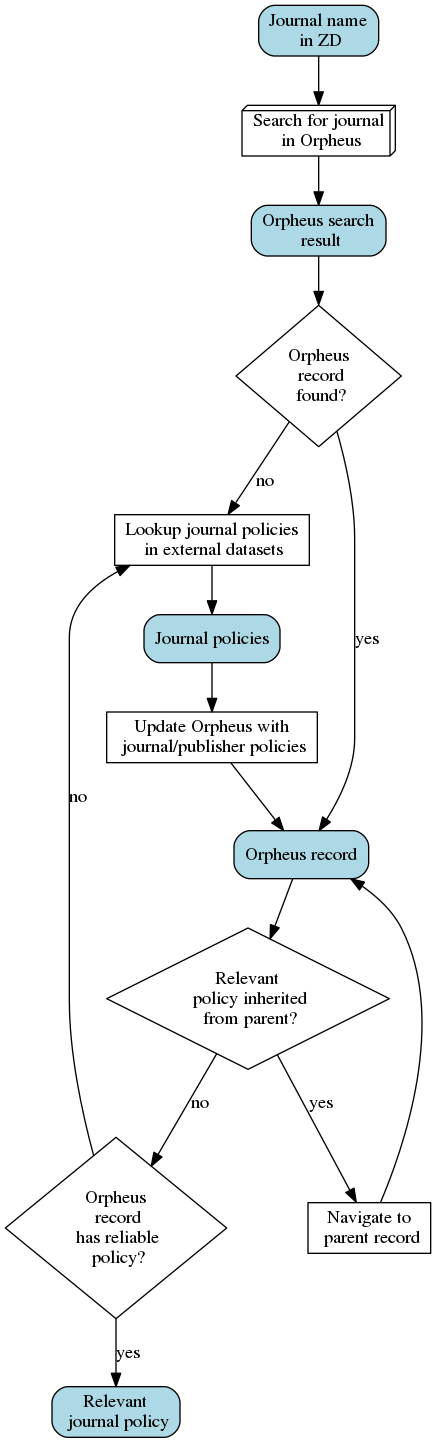
\includegraphics[width=0.48\textwidth]{initial-use}
  \end{center}
  \caption{Workflow for integrating Orpheus curation and RCUK/COAF funding decision.}
  \label{figure-general-use}
\end{figure}
%\end{wrapfigure}

Figure \vref{figure-general-use} maps the workflow for general use and curation of Orpheus. Members of the Open Access team making decisions on funding should use Orpheus as the first resouce to find out a journal's OA status, embargo period, APC value and any other relevant journal policy.

If a record for the queried journal is not found in Orpheus (please bear in mind that the journal might be represented by a synonym), proceed as we have done in the past and search publisher websites, SHERPA RoMEO and other external sources instead. Once you have found data about the missing journal, please add it to Orpheus. Similarly, if the journal already exists in Orpheus, but the relevant policy is missing, please add it to the database once you have found it elsewhere.

If the relevant policy in Orpheus is linked to the publisher record instead of directly to the journal of interest, you will see the notice ``\textcolor{red}{[inherited from publisher: $<$publisher name$>$}''. In this case, instead of adding or editing policies at the journal level, it is more efficient to navigate to the publisher record and add/edit the policy there instead, because the corrected policy will then be inherited by all journals linked to that publisher record.

Problematic self-archiving (green) policies inherited from RoMEO are marked with a red cross (
\includegraphics{icon-no}). These policies cannot be trusted until an Orpheus editor has revised and translated its contents. Figures \vref{figure-journal-inheriting-from-romeo} and \vref{figure-journal-inheriting-from-romeo-after-translation} are an example of an Orpheus journal record with policies inherited from RoMEO before and after policy revision. These policies apply to 5 other journals (Journal of Cosmology and Astroparticle Physics;  Journal of Instrumentation;  Journal of Physics A: Mathematical and Theoretical;  Journal of Physics G: Nuclear and Particle Physics;  Journal of Statistical Mechanics: Theory and Experiment).

\begin{figure}
  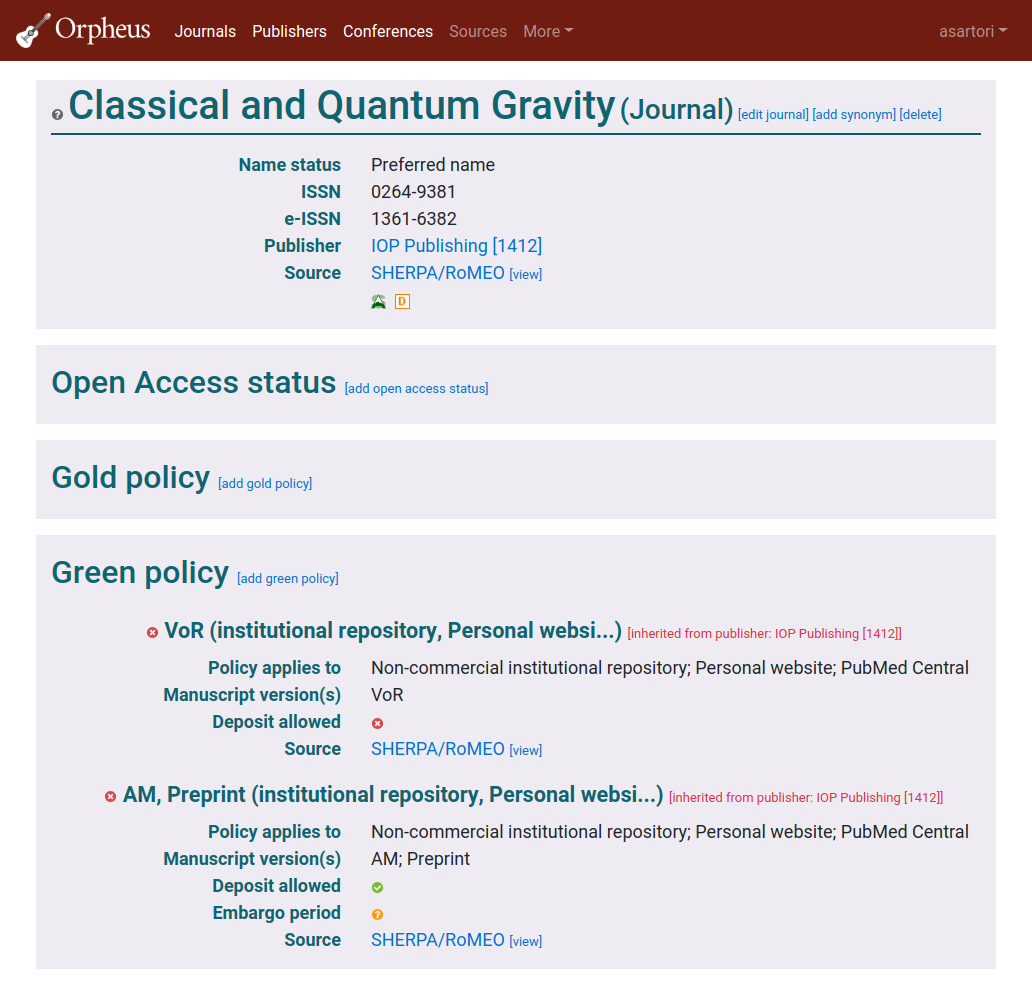
\includegraphics[width=\textwidth]{journal-inheriting-problematic-policies-from-romeo}
  \caption{Example of a journal with self-archiving policies inherited from RoMEO.}
  \label{figure-journal-inheriting-from-romeo}
\end{figure} 

\begin{figure}
  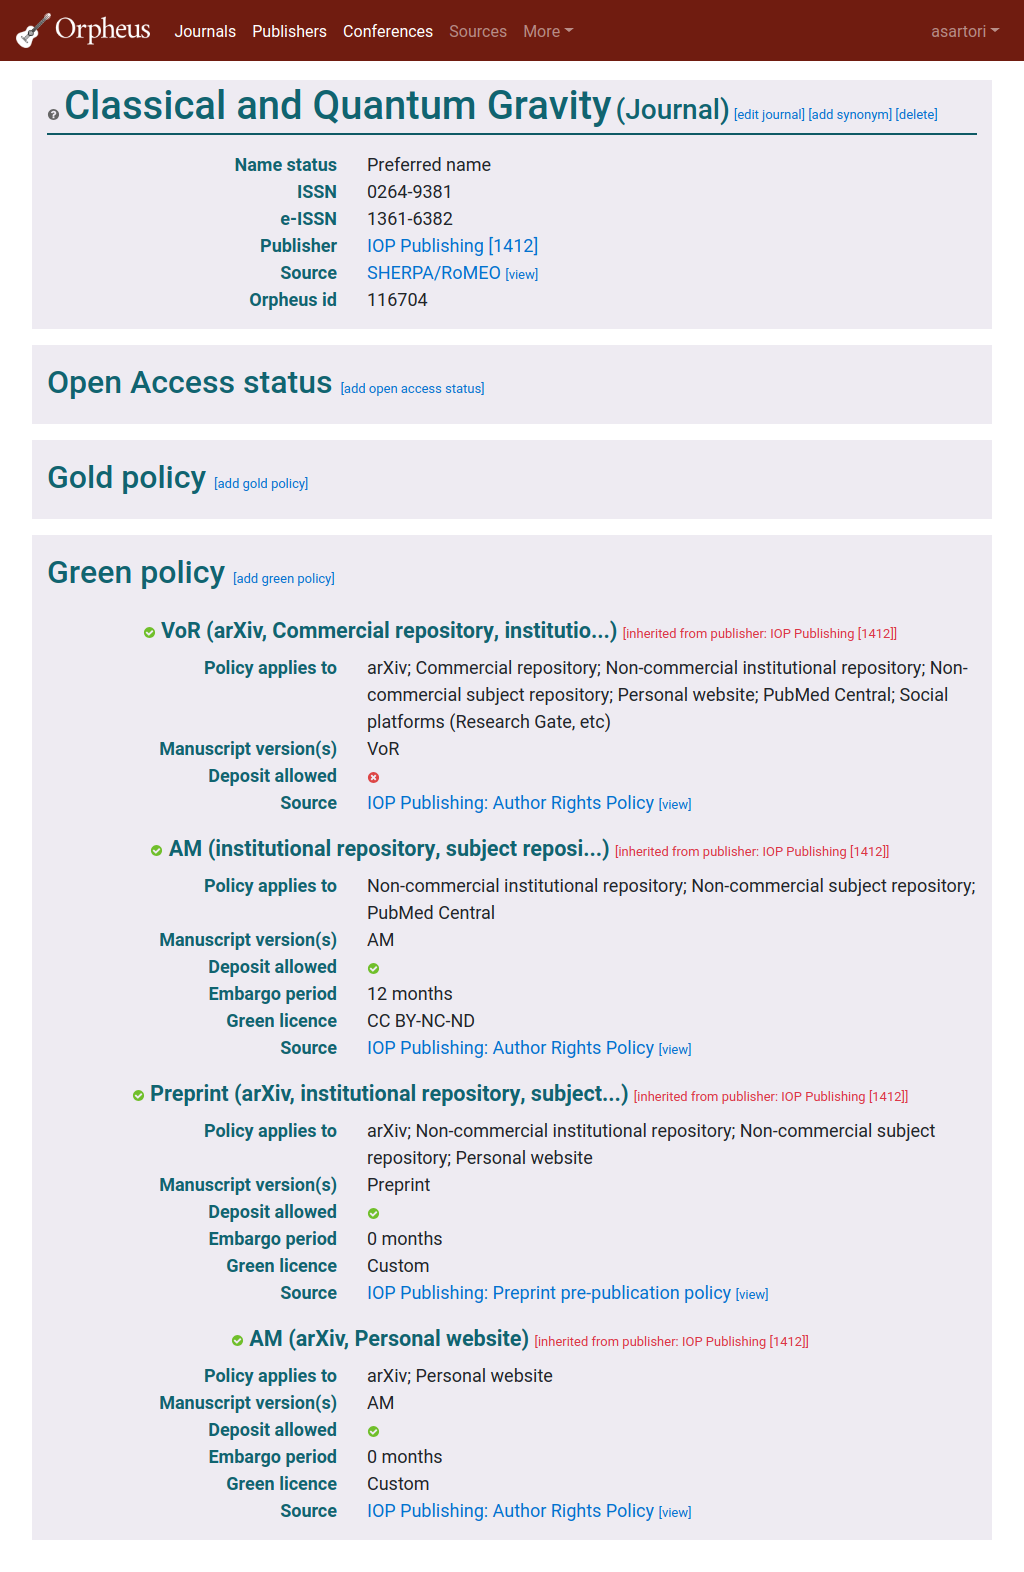
\includegraphics[width=\textwidth]{journal-inheriting-problematic-policies-from-romeo-after-translation}
  \caption{Journal shown in figure \vref{figure-journal-inheriting-from-romeo}, showing the effect of translation of RoMEO publisher policy.}
  \label{figure-journal-inheriting-from-romeo-after-translation}
\end{figure}


\section{Cambridge-specific features and integrations}

This section documents Orpheus features that are tailored for \href{https://www.repository.cam.ac.uk/}{Apollo}, the Cambridge institutional repository, and supporting infrastructure. It is probably only of interest to members of the University of Cambridge Office of Scholarly Communication.

\subsection{Integration with Zendesk (Orpheus lookup application)}

\software{Orpheus lookup} is a Zendesk application developed in collaboration with Agustina Martinez. The source code and documentation is available at \url{https://github.com/osc-cam/orpheus-lookup}.

The application allows \software{Zendesk} agents to query Orpheus for data on the journal associated to an individual Zendesk ticket. The following ticket fields are used for querying, in this order of precedence (i.e.\ if one of these fields is not empty, then it is used for querying and the next fields in the list are ignored):

\begin{enumerate}
 \item \#Apollo ISSN
 \item \#Apollo eISSN
 \item \#Journal title
\end{enumerate}

\begin{warn}
  Note that the value of these fields may change after ticket creation and \software{Orpheus lookup} always uses the current value of the field. Hence, the queried journal title may be distinct from what was recorded in the first Zendesk public comment (the one generated at ticket creation) as exemplified in \figt{\ref{fig-journal-title}}.
\end{warn}



\begin{figure}
  \begin{tikzpicture}
    \node[anchor=south west,inner sep=0] (image) at (0,0) {\fbox{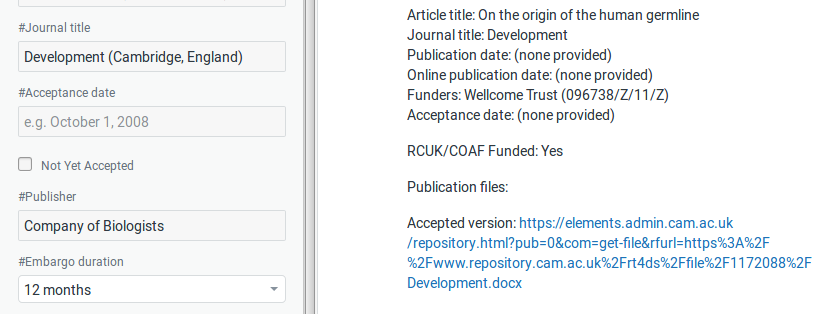
\includegraphics[width=\textwidth]{journal-title}}};
    % screenshot journals was taken by using Firefox inbuilt screenshot feature (https://support.mozilla.org/en-US/kb/firefox-screenshots) and selecting to take a screenshot of the whole screen after making the window just big enough to allow for the navigation bar to be properly displayed. This resulted in a screenshot sized 1038x1469 pixels
    \begin{scope}[x={(image.south east)},y={(image.north west)}]
%       \draw[help lines,xstep=.1,ystep=.1] (0,0) grid (1,1);
%       \draw[help lines,dashed,xstep=.05,ystep=.05] (0,0) grid (1,1);
%       \foreach \x in {0,1,...,9} { \node [red, anchor=north] at (\x/10,0) {0.\x}; }
%       \foreach \y in {0,1,...,9} { \node [red, anchor=east] at (0,\y/10) {0.\y}; }
       \annotatedFigureBox{0.025,0.75}{0.31,0.85}{A}
       \annotatedFigureBox{0.48,0.84}{0.7,0.91}{B}
    \end{scope}
  \end{tikzpicture}
  \caption{Example of Zendesk ticket in which field ``\#Journal title'' was modified by an ``Update on metadata received from Symplectic''. \abbv{A}{current value of field}; \abbv{B}{value of field at ticket creation}.}
  \label{fig-journal-title}
\end{figure}

\section{Getting help}

This manual should be the first point of call for help using and editing Orpheus. If you cannot find the answer to your question on these pages, please make a request for improved documentation (see \vref{section-bugs}).

You can also seek help from other users/editors in the \href{https://osc-cam.slack.com/messages/C8PJ1PDQS/}{Orpheus Slack channel}. If all else fails, you can try talking to the author or e-mailing him at \href{mailto:afs25@cam.ac.uk}{afs25@cam.ac.uk}.


\section{Reporting bugs, requesting new features}
\label{section-bugs}

Please use the \href{https://app.asana.com/0/648964409894394/board}{Orpheus' project board in Asana} to report any bugs, request new features, etc.



\printindex
\end{document}
